\subsection{Тематическое моделирование}

Как и в случае с электронными письмами Клинтон, в качестве модели используется латентное размещение Дирихле и такая же оценка качества --- перплексия.

В зависимости от параметра модели, отвечающего за количество тем у
распределения текстов, получилась следующая зависимость значения перплексии 
от количества тем:

\begin{figure}[H]
\centering
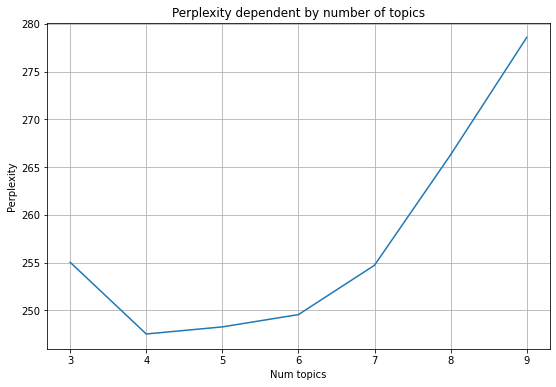
\includegraphics[scale=0.5]{pics/perplexity-2.png}
\caption{Перплексия модели в зависимости от количества тем в наборе $Enron$}
\end{figure}

Оптимальным значением получилось количество тем, равное 4. Ниже приведены примеры слов, принадлежащие каждой из 4 тем:

\begin{table}[H]
\centering
\begin{tabular}{ | l | l | l | }
\hline
Номер темы & Слова \\ \hline
1 & page, com, mail, please, new, click, order, 
\\ & free, receive, email \\ \hline
2 & please, enron, meet, thank, time, schedule, contact, 
\\ & attach, information, report \\ \hline
3 & get, know, send, subject, would, thank, week,
 \\ & message, let, think \\ \hline
4 & enron, company, market, page, would, state, issue, 
 \\ &  say, year, price \\ \hline 
\end{tabular}
\caption{Полученное описание тем в наборе $Enron$}
\end{table} 

Видим, что темы получились интерпретируемые, слова связаны между собой смыслом.

Как и ранее, для визуализации работы алгоритмы используется представление тем в
\textit{2D}:

\begin{figure}[H]
\centering
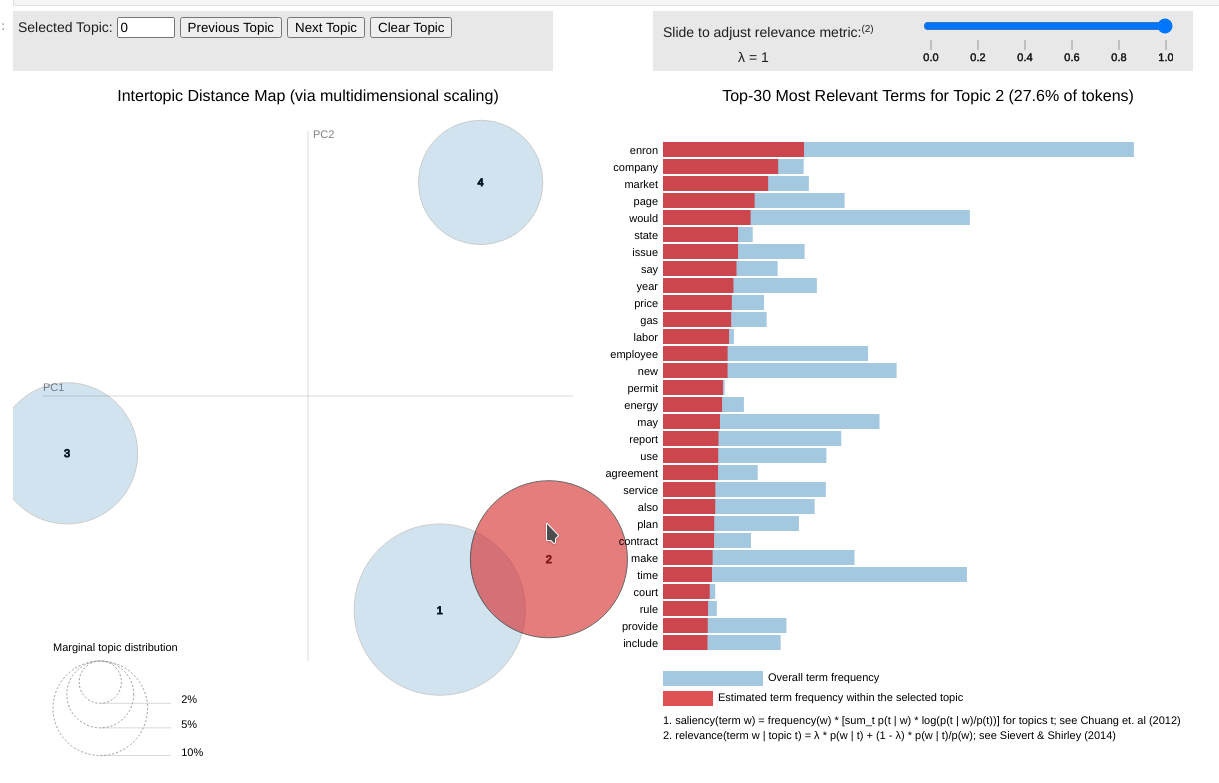
\includegraphics[scale=0.5]{pics/enron-lda-2d.png}
\caption{Визуализации тем для модели латентного размещения Дирихле в наборе $Enron$}
\end{figure}

К примеру, во второй теме сосредочены слова об $Enron$ и релевантные к деятельностьи компании термины.

